\documentclass[twocolumn,a4j]{jsarticle}
\setlength{\topmargin}{-20.4cm}
\setlength{\oddsidemargin}{-10.4mm}
\setlength{\evensidemargin}{-10.4mm}
\setlength{\textwidth}{18cm}
\setlength{\textheight}{26cm}

\usepackage[top=15truemm,bottom=20truemm,left=20truemm,right=20truemm]{geometry}
\usepackage[latin1]{inputenc}
\usepackage{amsmath}
\usepackage{amsfonts}
\usepackage{amssymb}
\usepackage[dvipdfmx]{graphicx}
\usepackage[hang,small,bf]{caption}
\usepackage[subrefformat=parens]{subcaption}
\usepackage[dvipdfmx]{color}
\usepackage{listings}
\usepackage{listings,jvlisting}
\usepackage{geometry}
\usepackage{framed}
\usepackage{color}
\usepackage[dvipdfmx]{hyperref}
\usepackage{ascmac}
\usepackage{enumerate}
\usepackage{tabularx}
\usepackage{cancel}
\usepackage{scalefnt}
\usepackage{overcite}
\usepackage{otf}
\usepackage{multicol}

\renewcommand{\figurename}{Fig.}
\renewcommand{\tablename}{Table }

\lstset{
basicstyle={\ttfamily},
identifierstyle={\small},
commentstyle={\smallitshape},
keywordstyle={\small\bfseries},
ndkeywordstyle={\small},
stringstyle={\small\ttfamily},
frame={tb},
breaklines=true,
columns=[l]{fullflexible},
xrightmargin=0zw,
xleftmargin=3zw,
numberstyle={\scriptsize},
stepnumber=1,
numbersep=1zw,
lineskip=-0.5ex
}

% キャプション後ろのダブルコロンを消す
\makeatletter
\long\def\@makecaption#1#2{%
  \vskip\abovecaptionskip
  \iftdir\sbox\@tempboxa{#1\hskip1zw#2}%
    \else\sbox\@tempboxa{#1 #2}%
  \fi
  \ifdim \wd\@tempboxa >\hsize
    \iftdir #1\hskip1zw#2\relax\par
      \else #1 #2\relax\par\fi
  \else
    \global \@minipagefalse
    \hbox to\hsize{\hfil\box\@tempboxa\hfil}%
  \fi
  \vskip\belowcaptionskip}
\makeatother

% タイトル
\makeatletter
\def\@maketitle
{
\begin{center}
{\LARGE \@title \par}
\end{center}
\begin{flushright}
{\large \@date 報告書 No.25}\\
{\large M1 \@author}
\end{flushright}
\par\vskip 1.5em
}
\makeatother

\author{来代 勝胤}
\title{令和4年度 4月 第2週 報告書}
\date{2022/4/11}

\begin{document}
\columnseprule=0.1mm
\maketitle

\section*{報告内容}
\begin{enumerate}[1.]
  \item 数値シミュレーションの作成
  \item 今後の予定
\end{enumerate}

\section{数値シミュレーションの作成}

\subsection{流れ構造}
回転円盤近傍の流体を考える.
静止する板があり,遠く離れた距離に一定の速度で回転する円盤がある.
円盤近くの流体は遠心力によって外側へ投げ出される.
一方で,静止板付近の粒子の周速の減少に伴い,
遠心力は大幅に減少するが,半径方向の圧力勾配は変わらないため
静止壁付近の流体が内側に流れることによって補完される.

\begin{figure}[htbp]
  \footnotesize
  \begin{center}
    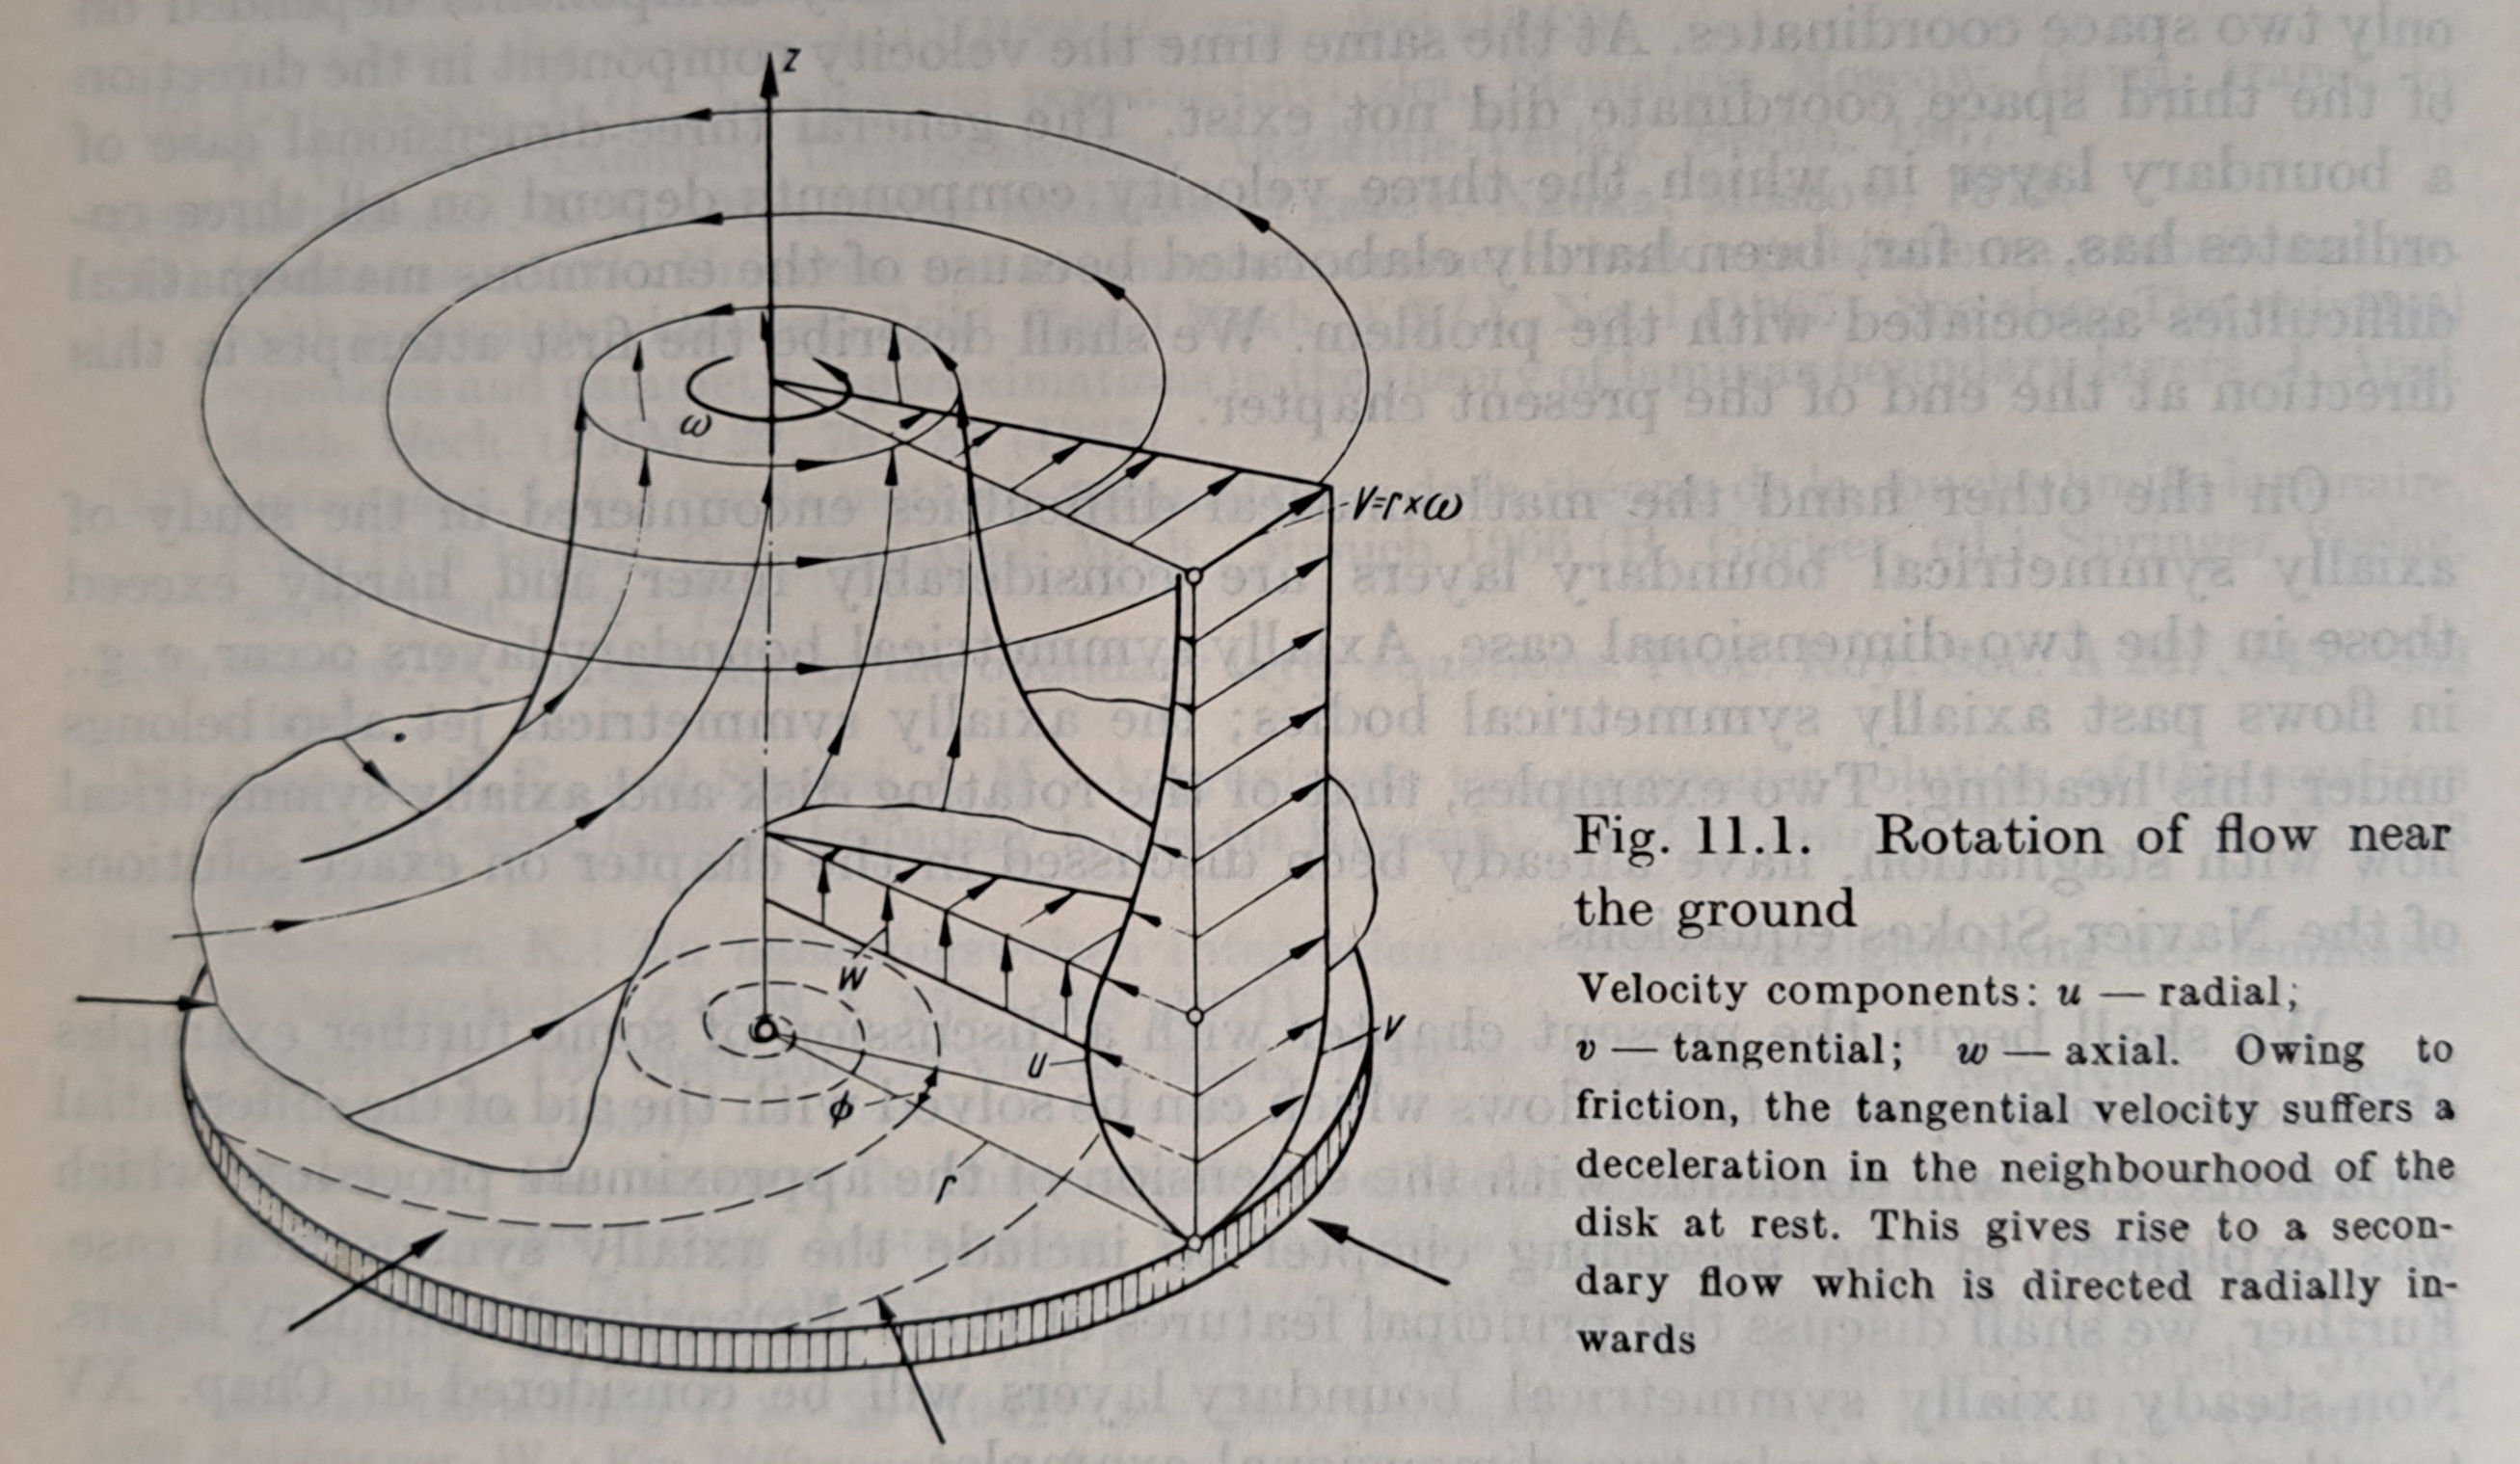
\includegraphics[width=80mm]{../images/Boundary-Layer_Theory_Fig.11.1.jpg}
    \caption{Rotation of flow near the ground ([1] P.226)}
  \end{center}
\end{figure}

\subsection{数値モデル}

\begin{table}[hbtp]
  \label{table:data_type}
  \caption{モデルの条件}
  \centering
  \begin{tabular}{ c | c }
    \hline
    円柱極座標系     & $r, \phi, z$ \\ \hline
    静止壁の位置     & $z = 0$      \\ \hline
    回転壁の回転速度 & $\omega$     \\ \hline
    半径方向速度     & $u$          \\ \hline
    周方向速度       & $v$          \\ \hline
    軸方向速度       & $w$          \\ \hline
  \end{tabular}
\end{table}

\subsection*{【境界条件】}
\begin{table}[hbtp]
  \centering
  \begin{tabular}{ c c c c }
    $z=0$      & $u=0$ & $v=0$        & $w=0$ \\
    $z=\infty$ & $u=0$ & $v=r \omega$ &       \\
  \end{tabular}
\end{table}

\newpage

\subsection*{【無次元座標】}
\begin{eqnarray*}
  \zeta &=& z \sqrt{\frac{\omega}{\nu}}\\
  u &=& r \omega F \left(\zeta\right)\\
  v &=& r \omega G \left(\zeta\right)\\
  w &=& \sqrt{\nu \omega} H \left(\zeta\right)
\end{eqnarray*}

\subsection*{【関数表】}

\begin{figure}[htbp]
  \footnotesize
  \begin{center}
    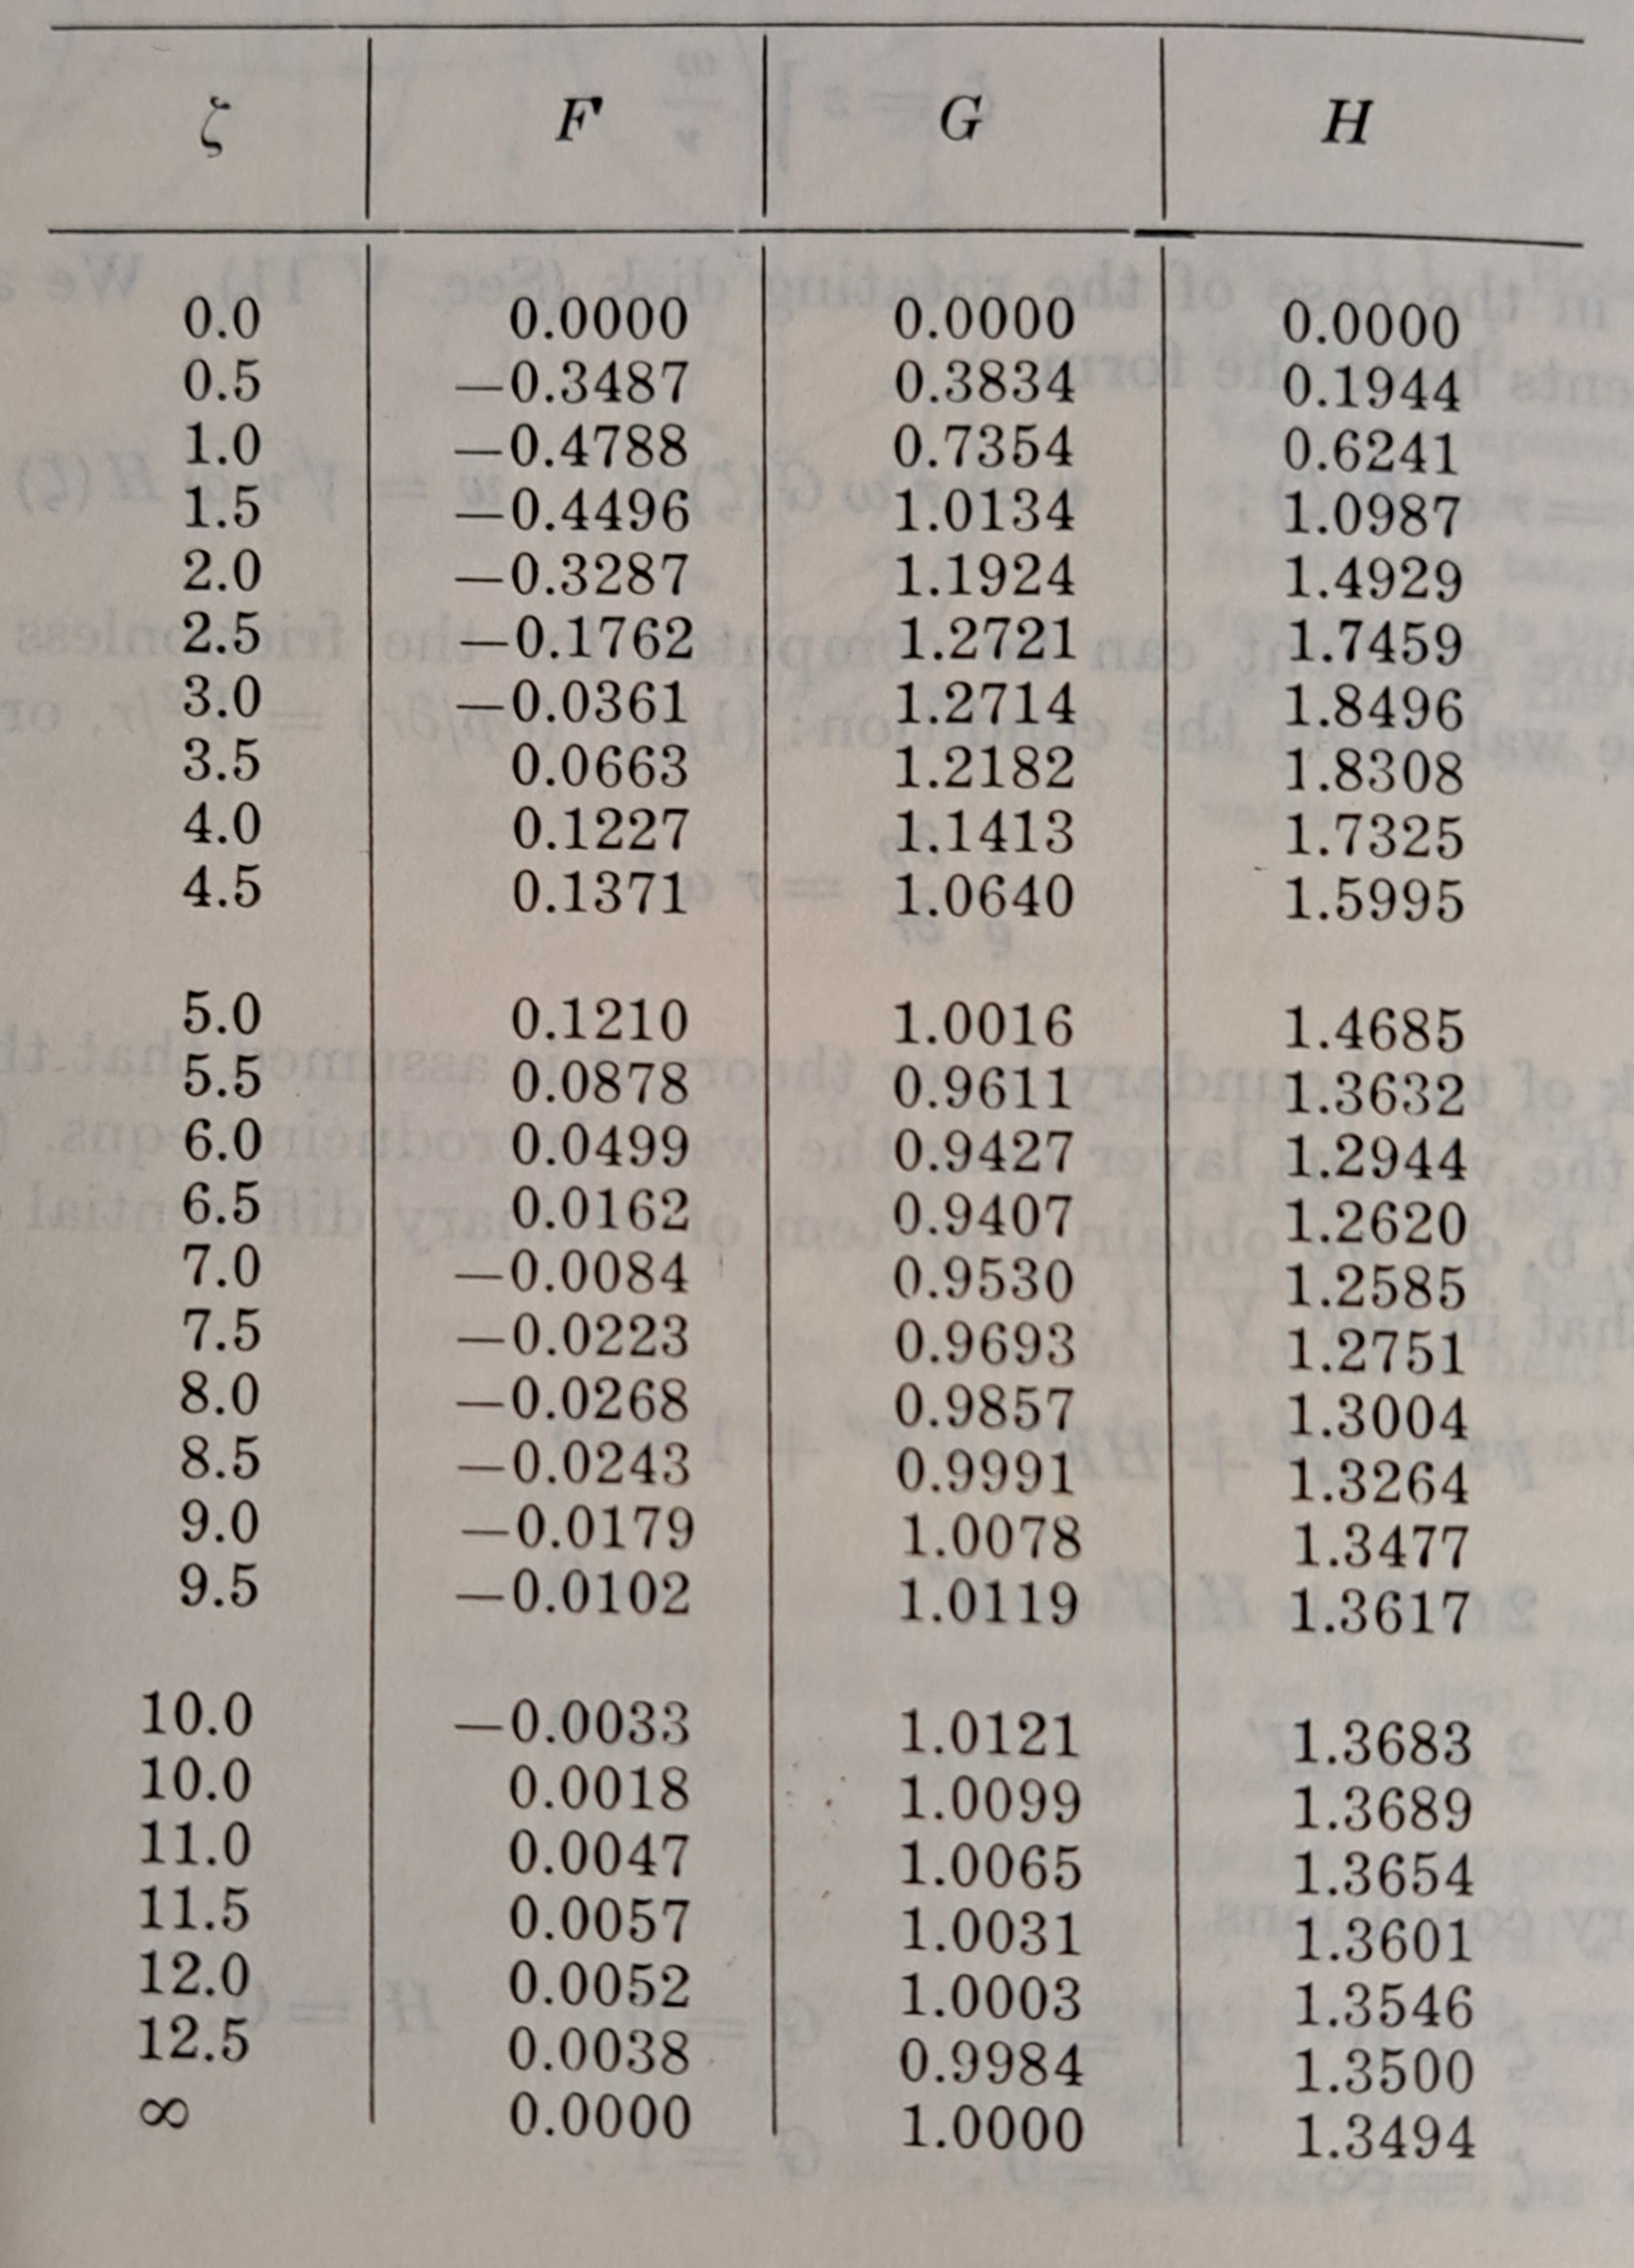
\includegraphics[width=60mm]{../images/function_table.jpg}
    \caption{Rotation of flow near the ground ([1] P.228)}
    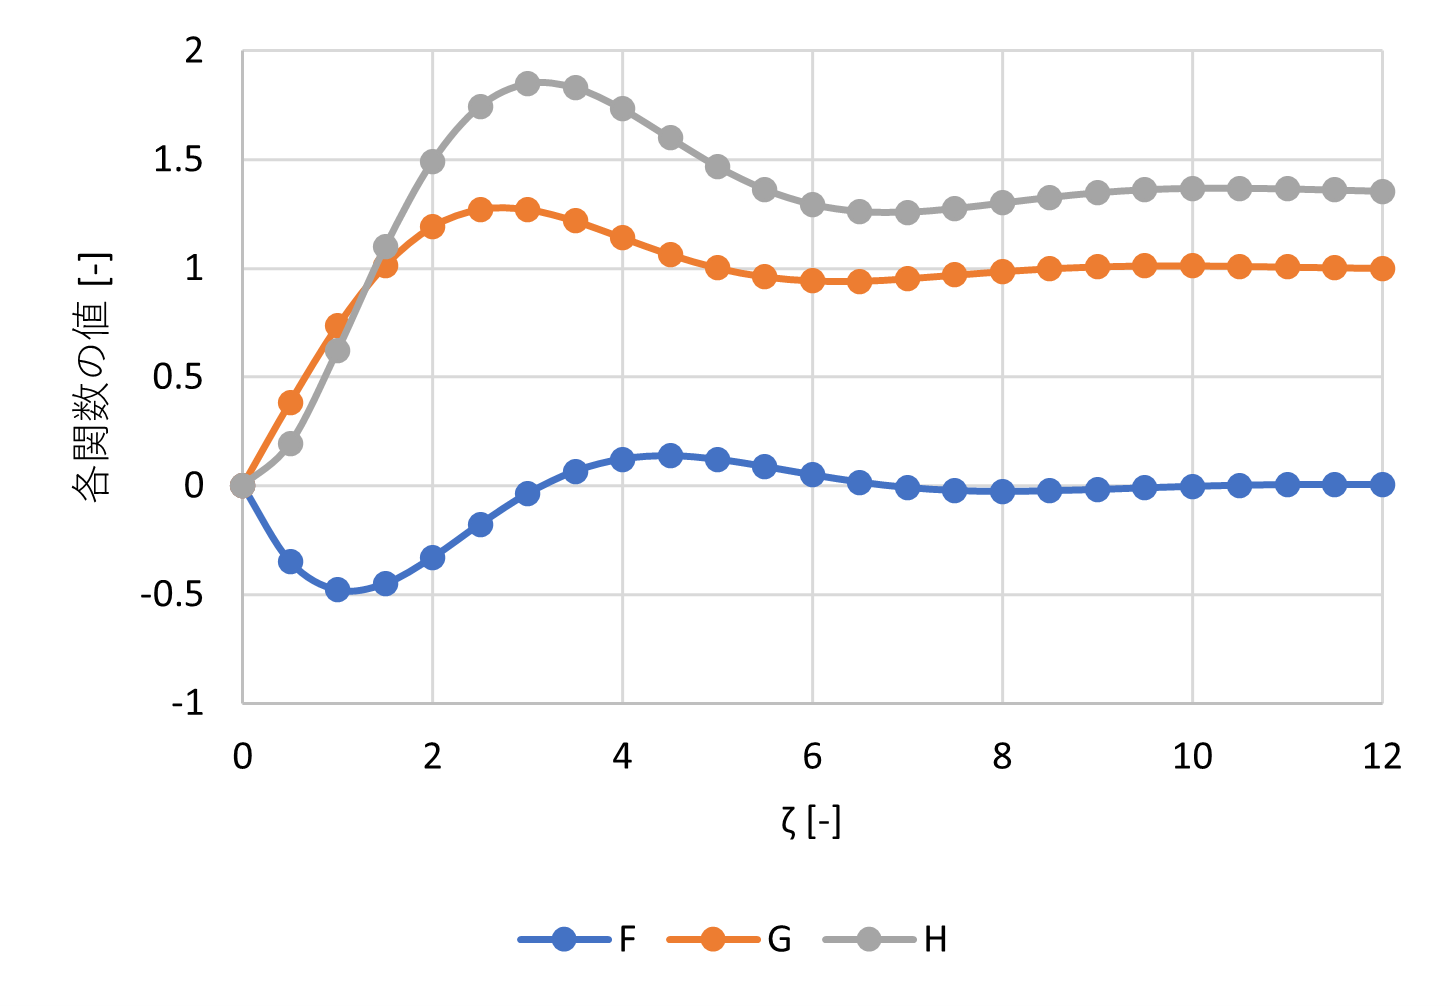
\includegraphics[width=70mm]{../images/function_graph.png}
    \caption{Graph of function table}
  \end{center}
\end{figure}

\section{今後の予定}
\begin{itemize}
  \item 流れの数値シミュレーション
  \item PTV解析の適用
\end{itemize}

\end{document}